\chapter{Context of the work}
\minitoc
\newpage

\setcounter{secnumdepth}{0} % Set the section counter to 0 so next section is not counted in toc
% ----------------------- Introduction ----------------------- %
\section{Introduction}
This chapter introduces the general context of this report. We start by
stating the problem which led to the realization of the project. Then we suggest a solution to these problems. Finally, we define the methodology we've followed to carry out our work.

\setcounter{secnumdepth}{2} % Resume counting the sections for the toc with a depth of 2 (Sections and sub-sections)
% ----------------------------------- SECTIONS (v) ----------------------------------- %
% ----------------------- Stating the problem ----------------------- %
\section{Stating the problem}
The focal point revolves around addressing the following inquiry: "How can we establish a \glsxtrfull{soc} to bolster our organization's defense against cyber threats?"
This question encapsulates the core challenge faced by our security team—ensuring continuous monitoring, analysis, and response capabilities to safeguard against evolving cyber risks.
The end goal is to fortify our organization's security posture and mitigate the impact of potential security incidents.

% ----------------------- Proposed solution ----------------------- %
\section{Proposed solution}
In response to the identified challenge, we present a comprehensive solution centered around the establishment of a \glsxtrshort{soc}. Drawing upon a robust framework encompassing cutting-edge tools and technologies, our solution enables continuous monitoring, analysis, and response to cyber threats. By integrating advanced threat detection mechanisms and proactive incident response protocols, our SoC implementation seeks to fortify our organization's defense against cyber risks and safeguard critical assets.

% ----------------------- Development Methodology ----------------------- %
\section{Development Methodology}
\subsection{Kanban}
Kanban is all about visualizing your work, limiting work in progress, and
maximizing efficiency (or flow). Kanban teams focus on reducing the time a
project takes from start by using a Kanban board to continuously improve
their flow of work. To explain more in details, Kanban is based on a con-
tinuous workflow structure that keeps teams nimble and ready to adapt to
changing priorities. Work items —represented by cards— are organized on
the board where they flow from one stage of the workflow or column to the
next. Common workflow stages are To Do, In Progress, In Review, and
Done.

\begin{figure}[H]
    \centering
    \makebox[\textwidth]{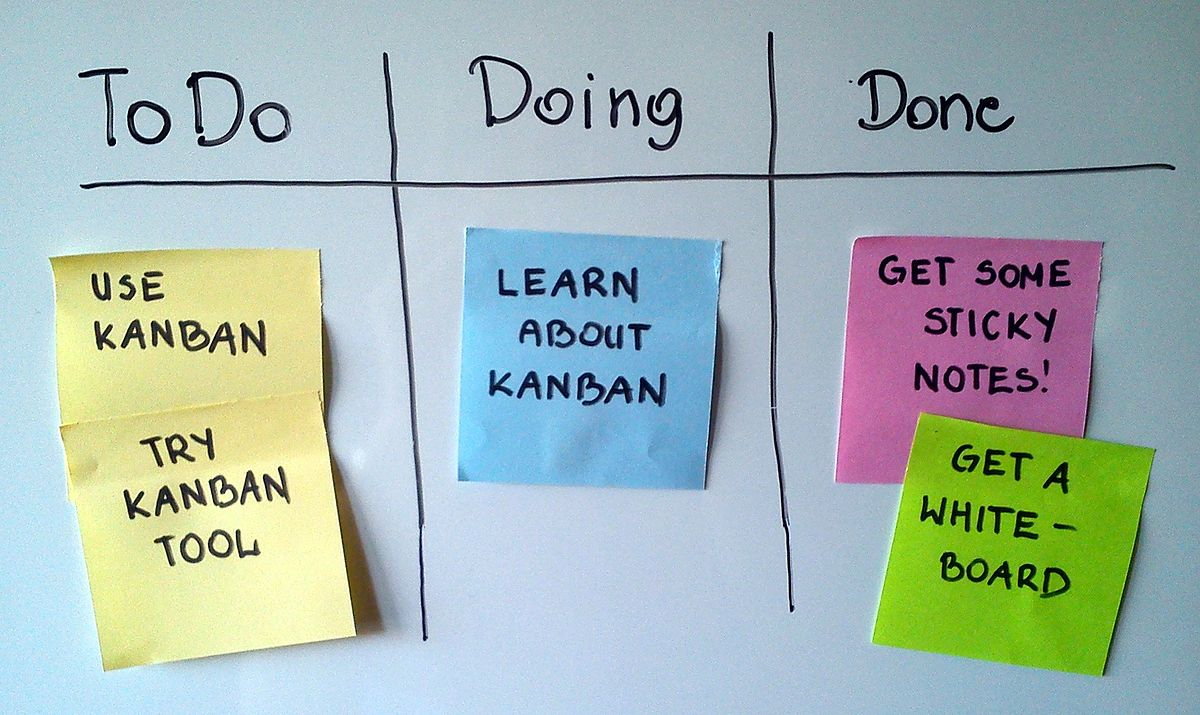
\includegraphics[width=\linewidth]{src/assets/images/simple-kanban-board.jpg}}
    \caption{Image of a Kanban board}
    \label{fig:kanban-board}
\end{figure}

\subsection{The choice for our project}
Since this project is quite susceptible to change, we decided to use the Kanban methodology. The latter is very flexible and allows us to adapt to the changes that may occur. This means delivering the project in a shorter time.

% ----------------------------------- SECTIONS (^) ----------------------------------- %

\setcounter{secnumdepth}{0} % Set the section counter to 0 so next section is not counted in toc
% ----------------------- Conclusion ----------------------- %
\section{Conclusion}
In this chapter, we've laid the groundwork for our exploration into establishing a \glsxtrshort{soc}. Beginning with the identification of the central challenge of enhancing our organization's cybersecurity posture, we've proposed a comprehensive solution focused on the implementation of a SoC. Through the integration of cutting-edge tools and technologies, our SoC aims to provide continuous monitoring, analysis, and response capabilities to mitigate cyber threats effectively. As we progress to the next chapter, we will delve into the datasets and the preparatory steps undertaken to facilitate the implementation of our SoC solution.

